% !TeX program = xelatex
\documentclass[a4paper,10pt]{article}

% ============================================================================
% សន្លឹកកិច្ចការសិស្ស ស-ខ្មៅ (Student Guided-Inquiry Worksheet - Grade 8 15.1 CIRC1)
% បរិបទ៖ ថ្នាក់រៀនគ្មានស្លាយ LCD – រុករកសញ្ញាណរង្វង់ និងប្រសព្វមេដ្យាទ័រ ២ ទំព័រ A4
% ============================================================================
\usepackage[a4paper, left=0.90cm, right=0.90cm, top=0.75cm, bottom=0.85cm, footskip=0.45cm]{geometry}
\usepackage{amsmath, amssymb}
\usepackage{unicode-math}
\usepackage{fontspec}
\usepackage{array, colortbl}
\usepackage[table]{xcolor}
\usepackage{enumitem}
\usepackage{pifont}
\usepackage{fancyhdr}
\usepackage{lastpage}
\usepackage{tikz}
\usepackage[most]{tcolorbox}
\usetikzlibrary{calc, arrows.meta, angles, quotes, decorations.markings, positioning, babel}

\makeatletter
\let\@expl@@@mark@update@singlecol@structures@@\relax
\makeatother

\providecommand{\NGSFindFonts}{%
  \IfFileExists{C:/Windows/Fonts/cambria.ttc}{%
    \def\NGSSysPath{C:/Windows/Fonts/}%
    \def\NGSUserPath{C:/Users/KIT/AppData/Local/Microsoft/Windows/Fonts/}%
  }{%
    \IfFileExists{./fonts/KhmerOSsiemreap.ttf}{\def\NGSSysPath{./fonts/}\def\NGSUserPath{./fonts/}}{%
    \IfFileExists{../fonts/KhmerOSsiemreap.ttf}{\def\NGSSysPath{../fonts/}\def\NGSUserPath{../fonts/}}{%
    \IfFileExists{../../fonts/KhmerOSsiemreap.ttf}{\def\NGSSysPath{../../fonts/}\def\NGSUserPath{../../fonts/}}{%
    \IfFileExists{../../../fonts/KhmerOSsiemreap.ttf}{\def\NGSSysPath{../../../fonts/}\def\NGSUserPath{../../../fonts/}}{%
    \IfFileExists{../../../../fonts/KhmerOSsiemreap.ttf}{\def\NGSSysPath{../../../../fonts/}\def\NGSUserPath{../../../../fonts/}}{%
    \IfFileExists{../../../../../fonts/KhmerOSsiemreap.ttf}{\def\NGSSysPath{../../../../../fonts/}\def\NGSUserPath{../../../../../fonts/}}{%
    \IfFileExists{../../../../../../fonts/KhmerOSsiemreap.ttf}{\def\NGSSysPath{../../../../../../fonts/}\def\NGSUserPath{../../../../../../fonts/}}{%
      \def\NGSSysPath{../../../../../../../fonts/}\def\NGSUserPath{../../../../../../../fonts/}%
    }}}}}}}%
  }%
}
\NGSFindFonts

\setmathfont[Path={\NGSSysPath}, FontIndex=1, Scale=1.02]{cambria.ttc}
\defaultfontfeatures{Ligatures=TeX}

\setmainfont[
  Path={\NGSUserPath},
  Extension=.ttf,
  Script=Khmer,
  BoldFont={KhmerOSsiemreap},
  BoldFeatures={FakeBold=1.8},
  ItalicFont={KhmerOSsiemreap},
  ItalicFeatures={FakeSlant=0.25},
  BoldItalicFont={KhmerOSsiemreap},
  BoldItalicFeatures={FakeBold=1.8, FakeSlant=0.25}
]{KhmerOSsiemreap}

\newfontfamily\muol[Path={\NGSUserPath}, Extension=.ttf, Script=Khmer]{KhmerOSmuollight}
\newfontfamily\TimesEn[Path={\NGSSysPath}, Extension=.ttf, BoldFont={timesbd}, ItalicFont={timesi}, BoldItalicFont={timesbi}]{times}

\XeTeXlinebreaklocale "km"
\XeTeXlinebreakskip = 0pt plus 1pt minus 0.1pt

\definecolor{panelgray}{gray}{0.94}
\definecolor{headgray}{gray}{0.86}

\pagestyle{fancy}
\fancyhf{}
\renewcommand{\headrulewidth}{0pt}
\fancyfoot[L]{\fontsize{8pt}{10pt}\selectfont អនុវិទ្យាល័យព្រះក្រសាំង \en{|} គណិតវិទ្យា ថ្នាក់ទី៨ \en{|} មេរៀនទី១៥ (១. សញ្ញាណរង្វង់ និងការកំណត់រង្វង់)}
\fancyfoot[R]{\fontsize{8.2pt}{10pt}\selectfont ទំព័រ \en{\thepage\ / \pageref{LastPage}}}

\setlength{\parindent}{0pt}
\setlength{\parskip}{0pt}
\setlength{\tabcolsep}{4pt}

\newcommand{\en}[1]{{\TimesEn #1}}
\newcommand{\enbf}[1]{{\TimesEn\textbf{#1}}}
\newcommand{\unit}[1]{\,\text{\en{#1}}}
\newcommand{\cnum}[1]{{\fontsize{10pt}{12pt}\selectfont\ding{\numexpr171+#1\relax}}}
\newcommand{\chk}{\tikz[baseline=-0.15ex]\draw[black, line width=0.8pt] (0,0) rectangle (0.25cm,0.25cm);}
\newcommand{\tri}[1]{\ensuremath{\triangle #1}}
\newcommand{\ang}[1]{\ensuremath{\angle #1}}
\newcommand{\arc}[1]{\ensuremath{\widehat{#1}}}
\newcommand{\dotline}[1]{\makebox[#1]{\dotfill}}

\newcolumntype{L}[1]{>{\raggedright\arraybackslash}p{#1}}
\newcolumntype{C}[1]{>{\centering\arraybackslash}p{#1}}

\tikzset{
  tk1/.style={postaction={decorate},decoration={markings,mark=at position 0.50 with {\draw[black, line width=0.90pt](0,-0.095)--(0,0.095);}}},
  tk2/.style={postaction={decorate},decoration={markings,
    mark=at position 0.45 with {\draw[black, line width=0.90pt](0,-0.095)--(0,0.095);},
    mark=at position 0.55 with {\draw[black, line width=0.90pt](0,-0.095)--(0,0.095);}}}
}

\newcommand{\secbar}[2]{%
  \vspace{3pt}
  \noindent\colorbox{headgray}{\parbox{\dimexpr\linewidth-2\fboxsep\relax}{%
    \vspace{1.5pt}{\muol\fontsize{9.5pt}{13.5pt}\selectfont #1}\hfill{\fontsize{8.5pt}{12pt}\selectfont\textbf{#2}}\vspace{1.5pt}%
  }}\par\vspace{3pt}
}

\begin{document}
\fontsize{9.5pt}{14.3pt}\selectfont

% ============================================================================
% ទំព័រទី១៖ ក្បាលសន្លឹកកិច្ចការ + E1 + E2 (ខ្នាតពិត 1:1) + E3
% ============================================================================
\begin{tcolorbox}[enhanced, sharp corners, colback=white, colframe=black, boxrule=1.0pt, top=4pt, bottom=4pt, left=6pt, right=6pt]
  \begin{center}
    {\muol\fontsize{10.5pt}{15pt}\selectfont សន្លឹកកិច្ចការសិស្ស — មេរៀនទី១៥៖ រង្វង់ \enbf{(}១. សញ្ញាណរង្វង់ និងការកំណត់រង្វង់\enbf{)}}\\[2pt]
    {\footnotesize សៀវភៅសិក្សាគោលថ្នាក់ទី៨ ទំព័រ ១៩៧--១៩៨ និង ២០៤ \en{|} រុករកដោយបន្ទាត់ក្រិត និងដែកឈាន (គ្មានស្លាយ \en{LCD})}
  \end{center}
  \vspace{2pt}
  \hrule height 0.5pt
  \vspace{4pt}
  ឈ្មោះសិស្ស៖ \dotline{5.3cm} ថ្នាក់៖ \dotline{2.0cm} ដៃគូទី៖ \dotline{2.0cm} កាលបរិច្ឆេទ៖ \dotline{3.3cm}
\end{tcolorbox}

% -------------------- ផ្នែកទី១៖ E1 ENGAGE --------------------
\secbar{ផ្នែកទី១ ៖ បេសកកម្មភ្ជាប់បញ្ហា \enbf{(E1 — Engage)} — បំណែកគែមចានបុរាណបាក់}{\en{3} នាទី (ទស្សន៍ទាយមុនរៀន)}

\begin{tcolorbox}[enhanced, sharp corners, colback=panelgray, colframe=black, boxrule=0.8pt, top=3pt, bottom=3pt, left=6pt, right=6pt]
  \begin{minipage}[c]{13.1cm}
    អ្នកបុរាណវិទ្យារកឃើញបំណែកគែមចានរាងរង្វង់មួយដែលបែកបាត់ផ្នែកផ្ចិតកណ្ដាល ដោយដៅចំណុចគែមបី $A, B$ និង $C$ ដូចរូបខាងស្ដាំ ។ ដើម្បីគូសស្ដាររង្វង់ដើមឡើងវិញ តើវិធីណារកផ្ចិត $O$ បានត្រឹមត្រូវជានិច្ច?\\[2pt]
    $\bullet$ \textbf{ការទស្សន៍ទាយដំបូងរបស់ប្អូន៖}\quad
    \chk\ មតិទី១៖ យកចំណុចកណ្ដាលនៃអង្កត់ $AC$ ជាផ្ចិត $O$\\[1.5pt]
    \hspace*{4.55cm}\chk\ មតិទី២៖ សង់ប្រសព្វមេដ្យាទ័រនៃអង្កត់ $AB$ និង $BC$\quad \chk\ មិនទាន់ប្រាកដ
  \end{minipage}\hfill
  \begin{minipage}[c]{5.2cm}
    \centering
    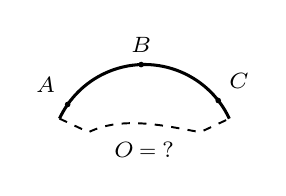
\begin{tikzpicture}[scale=0.68, every node/.style={font=\footnotesize, text=black}]
      \coordinate (O) at (2.0,0.4);
      \fill[white] (O) ++(25:1.75) arc (25:155:1.75) -- ($(O)+(155:1.15)$) .. controls (1.6,1.2) and (2.4,1.0) .. ($(O)+(25:1.15)$) -- cycle;
      \draw[black, line width=1.1pt] (O) ++(25:1.75) arc (25:155:1.75);
      \draw[black, line width=0.7pt, dashed] ($(O)+(155:1.75)$) -- ($(O)+(155:1.15)$) .. controls (1.6,1.2) and (2.4,1.0) .. ($(O)+(25:1.15)$) -- ($(O)+(25:1.75)$);
      \fill[black] ($(O)+(145:1.75)$) circle (1.5pt) node[above left=1pt] {$A$};
      \fill[black] ($(O)+(92:1.75)$) circle (1.5pt) node[above=1pt] {$B$};
      \fill[black] ($(O)+(38:1.75)$) circle (1.5pt) node[above right=1pt] {$C$};
      \node at (2.0,0.55) {$O=?$};
    \end{tikzpicture}
  \end{minipage}
\end{tcolorbox}

% -------------------- ផ្នែកទី២៖ E2 EXPLORE --------------------
\secbar{ផ្នែកទី២ ៖ ការរុករកតាមខ្នាតពិត \enbf{1:1} និងប្រសព្វមេដ្យាទ័រ \enbf{(E2 — Explore)}}{\en{11} នាទី (ពិភាក្សាដៃគូ)}

\begin{tcolorbox}[enhanced, sharp corners, colback=white, colframe=black, boxrule=0.85pt, top=4pt, bottom=4pt, left=6pt, right=6pt]
  \begin{minipage}[c]{9.0cm}
    \centering
    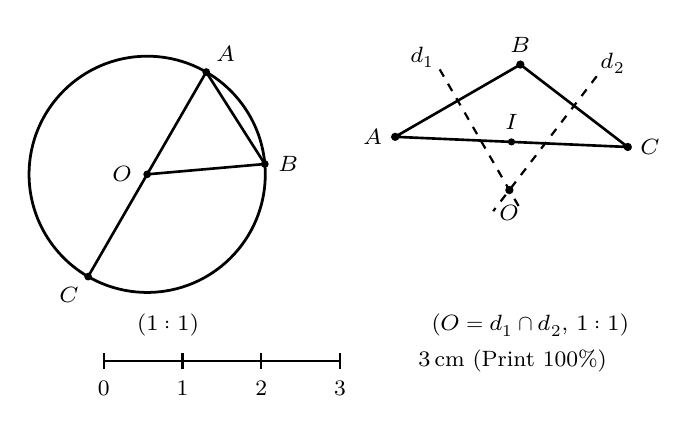
\begin{tikzpicture}[x=1cm, y=1cm, every node/.style={font=\footnotesize, text=black}]
      % រូប ក៖ រង្វង់ C(O, 1.5 cm) ខ្នាតពិត 1:1
      \coordinate (O) at (1.75,1.85);
      \draw[black, line width=1.0pt] (O) circle (1.50);
      \coordinate (A) at ($(O)+(60:1.50)$);
      \coordinate (C) at ($(O)+(240:1.50)$);
      \coordinate (B) at ($(O)+(5:1.50)$);
      \draw[black, line width=0.95pt] (A)--(C) (A)--(B) (O)--(B);
      \fill[black] (O) circle (1.4pt) node[left=2pt] {$O$};
      \fill[black] (A) circle (1.4pt) node[above right=0.5pt] {$A$};
      \fill[black] (B) circle (1.4pt) node[right=1.5pt] {$B$};
      \fill[black] (C) circle (1.4pt) node[below left=0.5pt] {$C$};
      \node[anchor=north] at (1.75,0.20) {\textbf{រូប ក} ($1:1$)};

      % រូប ខ៖ បីចំណុច A, B, C លើរង្វង់កាំ 1.6 cm ខ្នាតពិត 1:1
      \begin{scope}[shift={(4.45,0)}]
        \coordinate (O2) at (1.90,1.65);
        \coordinate (P1) at ($(O2)+(155:1.60)$);
        \coordinate (P2) at ($(O2)+(85:1.60)$);
        \coordinate (P3) at ($(O2)+(20:1.60)$);
        \coordinate (Iac) at ($(P1)!0.5!(P3)$);
        \coordinate (Mab) at ($(P1)!0.5!(P2)$);
        \coordinate (Mbc) at ($(P2)!0.5!(P3)$);
        \draw[black, line width=0.95pt] (P1)--(P2)--(P3)--cycle;
        \draw[black, line width=0.8pt, dashed] ($(Mab)!-0.35!(O2)$)--($(Mab)!1.25!(O2)$);
        \draw[black, line width=0.8pt, dashed] ($(Mbc)!-0.35!(O2)$)--($(Mbc)!1.25!(O2)$);
        \node[above left=0.5pt] at ($(Mab)!-0.25!(O2)$) {$d_1$};
        \node[above right=0.5pt] at ($(Mbc)!-0.25!(O2)$) {$d_2$};
        \fill[black] (P1) circle (1.5pt) node[left=1pt] {$A$};
        \fill[black] (P2) circle (1.5pt) node[above=1pt] {$B$};
        \fill[black] (P3) circle (1.5pt) node[right=1pt] {$C$};
        \fill[black] (Iac) circle (1.3pt) node[above=1pt] {$I$};
        \fill[black] (O2) circle (1.5pt) node[below=2pt] {$O$};
        \node[anchor=north] at (1.90,0.20) {\textbf{រូប ខ} ($O = d_1\cap d_2$, $1:1$)};
      \end{scope}

      % បន្ទះក្រិតផ្ទៀងខ្នាតពិត 3 cm (Actual Size 100%)
      \draw[black, line width=0.9pt] (1.20,-0.52) -- (4.20,-0.52);
      \foreach \x/\lbl in {1.20/0, 2.20/1, 3.20/2, 4.20/3} {
        \draw[black, line width=0.8pt] (\x,-0.62) -- (\x,-0.42);
        \node[below=2pt] at (\x,-0.58) {\en{\lbl}};
      }
      \node[right=4pt] at (4.20,-0.52) {\footnotesize ខ្នាតពិត $\en{3\unit{cm}}$ (\en{Print 100\%})};
    \end{tikzpicture}
  \end{minipage}\hfill
  \begin{minipage}[c]{9.2cm}
    \textbf{១. ពិនិត្យរូប ក (ធាតុនៃរង្វង់ ទំ.១៩៧)៖}\\[1.5pt]
    $\bullet$ ប្រើបន្ទាត់ក្រិតវាស់៖ $OA =$ \dotline{1.0cm}$\unit{cm}$, $OB =$ \dotline{1.0cm}$\unit{cm}$, $OC =$ \dotline{1.0cm}$\unit{cm}$ (ហៅថា \textbf{កាំ} $r$) ។\\[1.5pt]
    $\bullet$ អង្កត់ផ្ចិត $AC =$ \dotline{1.1cm}$\unit{cm} = 2 \times$ \dotline{0.9cm} ។ អង្កត់ $AB$ ហៅថា \dotline{2.1cm} ។\\[3pt]
    \textbf{២. ចំនួនរង្វង់កាត់តាម ១ ចំណុច និង ២ ចំណុច (ទំ.១៩៧--១៩៨)៖}\\[1.5pt]
    $\bullet$ កាត់តាម ១ ចំណុច $A$៖ គូសបានរង្វង់ \dotline{2.6cm} ។\\[1.5pt]
    $\bullet$ កាត់តាម ២ ចំណុច $A, B$ ($OA=OB$)៖ ផ្ចិតទាំងអស់ស្ថិតលើបន្ទាត់ \dotline{2.4cm} នៃអង្កត់ $AB$ (គូសបាន \dotline{2.1cm}) ។\\[3pt]
    \textbf{៣. ពិនិត្យរូប ខ (អន្ទាក់មតិទី១ ទល់នឹងប្រសព្វមេដ្យាទ័រ $O$)៖}\\[1.5pt]
    $\bullet$ វាស់ពីចំណុចកណ្ដាល $I$ នៃ $AC$៖ $IA \approx 1.48\unit{cm}$ តែ $IB \approx$ \dotline{1.1cm}$\unit{cm} \Rightarrow$ តើ $I$ ជាផ្ចិតរង្វង់ឬទេ? \chk\ មែន \quad \chk\ មិនមែន!\\[1.5pt]
    $\bullet$ វាស់ពីប្រសព្វមេដ្យាទ័រ $O$៖ $OA = OB = OC =$ \dotline{1.1cm}$\unit{cm}$ ។ ចូរចាក់ដែកឈានត្រង់ $O$ គូសរង្វង់កាត់តាម $A, B, C$ លើរូប ខ!\\[1.5pt]
    $\bullet$ \textbf{អន្ទាក់ទី២៖} បើ $A, B, C$ រត់ត្រង់គ្នាលើបន្ទាត់តែមួយ មេដ្យាទ័រ $d_1$ និង $d_2$ \dotline{1.8cm} គ្នា $\Rightarrow$ គូសរង្វង់បានចំនួន \dotline{1.3cm} ។
  \end{minipage}
\end{tcolorbox}

% -------------------- ផ្នែកទី៣៖ E3 EXPLAIN --------------------
\secbar{ផ្នែកទី៣ ៖ សំយោគនិយមន័យ ទ្រឹស្ដីបទ និងធនាគារហេតុផល \enbf{(E3 — Explain)}}{\en{6} នាទី (ទំ.១៩៧--១៩៨)}

\begin{tcolorbox}[enhanced, sharp corners, colback=white, colframe=black, boxrule=0.95pt, top=3.5pt, bottom=3.5pt, left=6pt, right=6pt]
  $\bullet$ \textbf{និយមន័យរង្វង់ $C(O, r)$៖} សំណុំចំណុចក្នុងប្លង់ដែលមានចម្ងាយស្មើនឹង \dotline{1.1cm} ពីផ្ចិត $O$ ។ អង្កត់ធ្នូដែលកាត់តាមផ្ចិត $O$ ហៅថា \dotline{2.3cm} ($d =$ \dotline{1.1cm}) ។\\[2pt]
  $\bullet$ \textbf{ទ្រឹស្ដីបទ (ទំ.១៩៨)៖} តាមបីចំណុចដែល \dotline{3.8cm} គេអាចគូសបាន \dotline{2.6cm} ដែលកាត់តាមចំណុចទាំងនោះ ។\\[3pt]
  {\fontsize{8.9pt}{12.5pt}\selectfont
  \begin{tabular}{|L{3.55cm}|C{2.45cm}|L{3.55cm}|L{3.45cm}|L{4.00cm}|}
    \hline
    \cellcolor{headgray}\centering\textbf{\cnum{1} និយមន័យ $C(O,r)$} &
    \cellcolor{headgray}\centering\textbf{\cnum{2} អង្កត់ផ្ចិត-កាំ} &
    \cellcolor{headgray}\centering\textbf{\cnum{3} លក្ខណៈមេដ្យាទ័រ} &
    \cellcolor{headgray}\centering\textbf{\cnum{4} រង្វង់តាម ៣ ចំណុច} &
    \cellcolor{headgray}\centering\arraybackslash\textbf{\cnum{5} ទីតាំងរង្វង់ពីរ} \\[2pt]
    \hline
    $M \in C(O,r) \iff OM = r$ (ស្មើចម្ងាយពីផ្ចិត $O$) &
    $d = 2r$\par\vspace{2pt}$r = \dfrac{d}{2}$ &
    $O \in \text{មេដ្យាទ័រនៃ } AB \iff OA = OB$ &
    $A,B,C$ មិនរត់ត្រង់គ្នា $\Rightarrow \exists!\, C(O,r)$ ($O=d_1\cap d_2$) &
    ប៉ះក្រៅ៖ $AB=r_1+r_2$\par ប្រសព្វ៖ $|r_1-r_2|<AB<r_1+r_2$\par ដាច់គ្នា៖ $AB>r_1+r_2$ \\[2pt]
    \hline
  \end{tabular}}
\end{tcolorbox}

\newpage

% ============================================================================
% ទំព័រទី២៖ E4 លំហាត់គំរូបំពេញចន្លោះ + E5 ប្រតិបត្តិ & Exit Check + កិច្ចការផ្ទះ
% ============================================================================
\secbar{ផ្នែកទី៤ ៖ លំហាត់គំរូសម្រាយបញ្ជាក់តាមជំហាន \enbf{(E4 — Faded Worked Examples)}}{\en{10} នាទី (ទំ.១៩៨ និង ២០៤)}

\begin{tcolorbox}[enhanced, sharp corners, colback=white, colframe=black, boxrule=0.90pt, top=4pt, bottom=4pt, left=6pt, right=6pt, after skip=5pt]
  \begin{minipage}[c]{12.7cm}
    \textbf{គំរូទី១ (លំហាត់គំរូ ទំ.១៩៨ — ស្រាយថា ៣ ចំណុចមិនរត់ត្រង់គ្នាស្ថិតលើរង្វង់តែមួយ)៖}\\
    គេមានបីចំណុច $A, B$ និង $C$ មិនស្ថិតនៅលើបន្ទាត់តែមួយ ។ ស្រាយបញ្ជាក់ថា $A, B, C$ ស្ថិតនៅលើរង្វង់តែមួយគត់ ។\\[2pt]
    $\bullet$ គូសមេដ្យាទ័រ $MN$ នៃអង្កត់ $AC$ និងមេដ្យាទ័រ $PQ$ នៃអង្កត់ $AB$ ។\\[2pt]
    $\bullet$ ដោយ $A, B, C$ មិនរត់ត្រង់គ្នា មេដ្យាទ័រ $MN$ និង $PQ$ ប្រសព្វគ្នាត្រង់ចំណុច \dotline{1.0cm} តែមួយគត់៖\\
    \hspace*{0.4cm}-- ដោយ $O \in MN$ (មេដ្យាទ័រនៃ $AC$) គេបាន $OA =$ \dotline{1.2cm} (តាមហេតុផលលេខ \dotline{0.9cm}) ។\\
    \hspace*{0.4cm}-- ដោយ $O \in PQ$ (មេដ្យាទ័រនៃ $AB$) គេបាន $OA =$ \dotline{1.2cm} (តាមហេតុផលលេខ \dotline{0.9cm}) ។\\[2pt]
    $\bullet$ ដូចនេះ $OA = OB = OC = r \Rightarrow$ ចំណុច $A, B, C$ ស្ថិតនៅលើរង្វង់តែមួយគត់ $C(O, OA)$ (តាម \dotline{0.9cm}) ។
  \end{minipage}\hfill
  \begin{minipage}[c]{5.5cm}
    \centering
    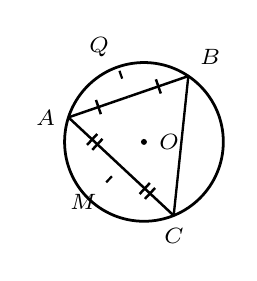
\begin{tikzpicture}[scale=0.72, every node/.style={font=\footnotesize, text=black}]
      \coordinate (O) at (1.7,1.5);
      \draw[black, line width=1.0pt] (O) circle (1.40);
      \coordinate (A) at ($(O)+(162:1.40)$);
      \coordinate (B) at ($(O)+(56:1.40)$);
      \coordinate (C) at ($(O)+(-68:1.40)$);
      \coordinate (Iab) at ($(A)!0.5!(B)$);
      \coordinate (Iac) at ($(A)!0.5!(C)$);
      \draw[black, line width=0.9pt, tk1] (A)--(Iab); \draw[black, line width=0.9pt, tk1] (Iab)--(B);
      \draw[black, line width=0.9pt, tk2] (A)--(Iac); \draw[black, line width=0.9pt, tk2] (Iac)--(C);
      \draw[black, line width=0.85pt] (B)--(C);
      \draw[black, line width=0.8pt, dashed] ($(Iab)!-0.4!(O)$)--($(O)!1.7!(Iab)$) node[above left=-1pt] {$Q$};
      \draw[black, line width=0.8pt, dashed] ($(Iac)!-0.4!(O)$)--($(O)!1.8!(Iac)$) node[below left=-1pt] {$M$};
      \fill[black] (O) circle (1.5pt) node[right=2pt] {$O$};
      \node[left=1pt] at (A) {$A$}; \node[above right=1pt] at (B) {$B$}; \node[below=1pt] at (C) {$C$};
    \end{tikzpicture}
  \end{minipage}
\end{tcolorbox}

\begin{tcolorbox}[enhanced, sharp corners, colback=panelgray, colframe=black, boxrule=0.90pt, top=4pt, bottom=4pt, left=6pt, right=6pt, after skip=5pt]
  \begin{minipage}[c]{12.7cm}
    \textbf{គំរូទី២ (លំហាត់ទី៦ ទំ.២០៤ — ស្រាយថា ៤ ចំណុចស្ថិតនៅលើរង្វង់តែមួយ)៖}\\
    គេមានត្រីកោណសម័ង្ស $\tri{ABC}$ (ជ្រុងស្មើគ្នា $AB=BC=CA=2a$) និង $I, J, K$ ជាចំណុចកណ្ដាលរៀងគ្នានៃ $AB, BC, CA$ ។ ស្រាយបញ្ជាក់ថាចំណុចទាំងបួន $B, I, K, C$ ស្ថិតនៅលើរង្វង់តែមួយដែលមានផ្ចិត $J$ ។\\[2pt]
    $\bullet$ ដោយ $J$ ជាចំណុចកណ្ដាលនៃ $BC \Rightarrow JB = JC = \dfrac{1}{2}BC =$ \dotline{1.2cm} ។\\[2pt]
    $\bullet$ ក្នុង $\tri{ABC}$ អង្កត់ $JI$ និង $JK$ ជា \textbf{បាតមធ្យម} (មេរៀនទី១៣)៖\\
    \hspace*{0.4cm}$JI = \dfrac{1}{2}AC =$ \dotline{1.2cm} \quad និង \quad $JK = \dfrac{1}{2}AB =$ \dotline{1.2cm} ។\\[2pt]
    $\bullet$ ដូចនេះ $JB = JI = JK = JC =$ \dotline{1.1cm} $\Rightarrow B, I, K, C$ ស្ថិតនៅលើរង្វង់តែមួយផ្ចិត \dotline{1.0cm} កាំ \dotline{1.0cm} (តាម \cnum{1}) ។
  \end{minipage}\hfill
  \begin{minipage}[c]{5.5cm}
    \centering
    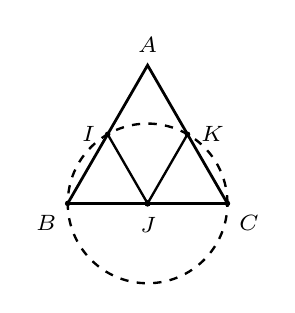
\begin{tikzpicture}[scale=0.78, every node/.style={font=\footnotesize, text=black}]
      \coordinate (B) at (0.2,0.4); \coordinate (C) at (2.8,0.4); \coordinate (A) at (1.5,2.65);
      \coordinate (J) at (1.5,0.4); \coordinate (I) at ($(A)!0.5!(B)$); \coordinate (K) at ($(A)!0.5!(C)$);
      \draw[black, line width=0.85pt, dashed] (J) circle (1.30);
      \draw[black, line width=1.0pt] (A)--(B)--(C)--cycle;
      \draw[black, line width=0.85pt] (J)--(I) (J)--(K);
      \fill[black] (J) circle (1.5pt) node[below=1.5pt] {$J$};
      \fill[black] (B) circle (1.3pt) node[below left=1pt] {$B$};
      \fill[black] (C) circle (1.3pt) node[below right=1pt] {$C$};
      \fill[black] (I) circle (1.3pt) node[left=1.5pt] {$I$};
      \fill[black] (K) circle (1.3pt) node[right=1.5pt] {$K$};
      \node[above=1pt] at (A) {$A$};
    \end{tikzpicture}
  \end{minipage}
\end{tcolorbox}

% -------------------- ផ្នែកទី៥៖ E5 EVALUATE --------------------
\secbar{ផ្នែកទី៥ ៖ លំហាត់ប្រតិបត្តិ និងតេស្តវាយតម្លៃរហ័ស \enbf{(E5 — Evaluate)}}{\en{10} នាទី (ទំ.១៩៨)}

\noindent
\begin{minipage}[t]{11.3cm}
  \begin{tcolorbox}[enhanced, sharp corners, colback=white, colframe=black, boxrule=0.90pt, top=4pt, bottom=4pt, left=5pt, right=5pt, equal height group=e5c1]
    \textbf{១. ប្រតិបត្តិ (ទំ.១៩៨)៖} គេឱ្យអង្កត់ $AB = 6\unit{cm}$ ។ ចូរបំពេញតារាងទីតាំងធៀបនៃរង្វង់ទាំងពីរតាម \cnum{5} និងគូសរង្វង់លើអ័ក្សក្រិតខាងក្រោម ($1\text{ ក្រឡា} = 1\unit{cm}$)៖\\[3pt]
    {\fontsize{8.8pt}{12.5pt}\selectfont
    \begin{tabular}{|L{3.65cm}|C{1.85cm}|L{4.35cm}|}
      \hline
      \cellcolor{headgray}\textbf{ករណីរង្វង់ទាំងពីរ} & \cellcolor{headgray}\textbf{$r_1 + r_2$} & \cellcolor{headgray}\textbf{ទីតាំងធៀបធៀបនឹង $AB=6\unit{cm}$} \\[2pt]
      \hline
      ក. $C(A,2\unit{cm})$ និង $C(B,4\unit{cm})$ & \dotline{1.3cm} & \dotline{3.9cm} \\[3pt]
      \hline
      ខ. $C(A,3\unit{cm})$ និង $C(B,5\unit{cm})$ & \dotline{1.3cm} & \dotline{3.9cm} \\[3pt]
      \hline
      គ. $C(A,1\unit{cm})$ និង $C(B,2\unit{cm})$ & \dotline{1.3cm} & \dotline{3.9cm} \\[3pt]
      \hline
    \end{tabular}}
    \begin{center}
      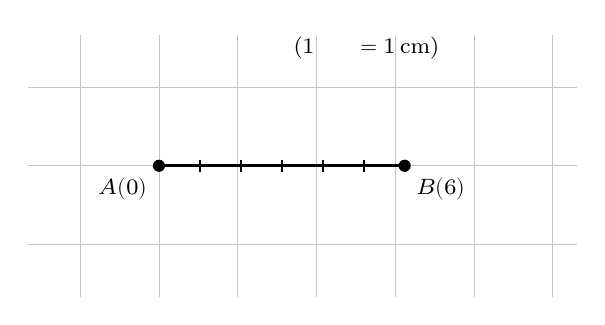
\begin{tikzpicture}[x=0.52cm, y=0.52cm, every node/.style={font=\footnotesize, text=black}]
        \draw[gray!45, very thin] (-3.2,-3.2) grid (10.2,3.2);
        \draw[black, line width=1.0pt] (0,0) -- (6,0);
        \foreach \x in {0,1,2,3,4,5,6} \draw[black, line width=0.7pt] (\x,-0.15)--(\x,0.15);
        \fill[black] (0,0) circle (2.2pt) node[below left=1pt] {$A(0)$};
        \fill[black] (6,0) circle (2.2pt) node[below right=1pt] {$B(6)$};
        \node[above=1pt] at (3,2.3) {\footnotesize គូសករណី ក និង គ ដោយដែកឈាន ($1\text{ ក្រឡា}=1\unit{cm}$)};
      \end{tikzpicture}
    \end{center}
  \end{tcolorbox}
\end{minipage}\hfill
\begin{minipage}[t]{7.4cm}
  \begin{tcolorbox}[enhanced, sharp corners, colback=white, colframe=black, boxrule=0.90pt, top=4pt, bottom=4pt, left=5pt, right=5pt, equal height group=e5c1]
    \textbf{២. បិទបេសកកម្ម E1 (ចានបុរាណ)៖}\\
    ដើម្បីរកផ្ចិតដើម $O$ នៃបំណែកចាន ត្រូវសង់ប្រសព្វនៃ \dotline{3.2cm} ទាំងពីរ ។\\[4pt]
    \textbf{៣. តេស្តរហ័ស (\en{Exit Check})៖}\\
    គេមានបីចំណុច $M, N, P$ ស្ថិតនៅលើបន្ទាត់ត្រង់តែមួយ ($MN=3\unit{cm}, NP=4\unit{cm}, MP=7\unit{cm}$) ។ តើគេអាចគូសរង្វង់កាត់តាម $M, N, P$ បានប៉ុន្មាន?\\[3pt]
    \chk\ \textbf{A.} មិនអាចគូសបាន ($0$ រង្វង់)\\[2.5pt]
    \chk\ \textbf{B.} បាន $1$ រង្វង់គត់\\[2.5pt]
    \chk\ \textbf{C.} បាន $2$ រង្វង់\\[2.5pt]
    \chk\ \textbf{D.} បានច្រើនរាប់មិនអស់\\[4pt]
    \textbf{ហេតុផល៖} ព្រោះមេដ្យាទ័រនៃ $MN$ និង $NP$៖\\
    \dotline{6.3cm}
  \end{tcolorbox}
\end{minipage}

% -------------------- ផ្នែកទី៦៖ កិច្ចការផ្ទះ --------------------
\vspace{5pt}
\begin{tcolorbox}[enhanced, sharp corners, colback=panelgray, colframe=black, boxrule=0.95pt, top=4pt, bottom=4pt, left=6pt, right=6pt]
  {\muol\fontsize{9.0pt}{13.5pt}\selectfont ផ្នែកទី៦ ៖ កិច្ចការផ្ទះ និងបណ្ដាំផ្ញើ (សៀវភៅសិក្សាគោល ទំព័រ ១៩៨ និង ២០៤ — ធ្វើក្នុងសៀវភៅលំហាត់)}\\[2.5pt]
  $\bullet$ \textbf{លំហាត់ទី៧ (ទំ.២០៤)៖} ចតុកោណ $ABCD$ មានអង្កត់ទ្រូងទាំងពីរកែងគ្នា ($AC \perp BD$) ហើយ $M, N, R, S$ ជាចំណុចកណ្ដាលរៀងគ្នានៃជ្រុង $AB, BC, CD, DA$ ។ ចូរស្រាយថា $MNRS$ ជាចតុកោណកែង រួចទាញថាចំណុចទាំងបួន $M, N, R, S$ ស្ថិតនៅលើរង្វង់តែមួយ ។\\[2pt]
  $\bullet$ \textbf{សំណង់ខ្នាតពិត៖} សង់រូប \textbf{ប្រតិបត្តិ ក, ខ, គ (ទំ.១៩៨)} តាមខ្នាតពិត $AB = 6\unit{cm}$ ដោយដែកឈានក្នុងសៀវភៅលំហាត់ និងអានមុនចំណុច \textbf{២.១ មុំផ្ចិត} (ទំ.១៩៩--២០០) ព្រមទាំងត្រៀមរ៉ាប់ព័រទ័រសម្រាប់ម៉ោងក្រោយ ។
\end{tcolorbox}

\end{document}
